\chapter{Existing Platforms}\label{chap:platforms}

To better understand what instruments people use when interacting with music,
it is helpful to examine existing solutions. Additionally, this research will provide insight
into the possible features to be implemented in the resulting application.

Firstly, streaming services are discussed, as the main aim of the thesis is to create a system for music streaming.
Then, other music-related portals are listed, as they offer alternative possibilities to engage with audio content, which
can also be beneficial for the future platform.
And lastly, products such as YouTube and TikTok are discussed, as they have proven to be a popular way to interact
with music as shown in~\ref{fig:discovery_methods}.

\begin{figure}[htbp]
    \centering
    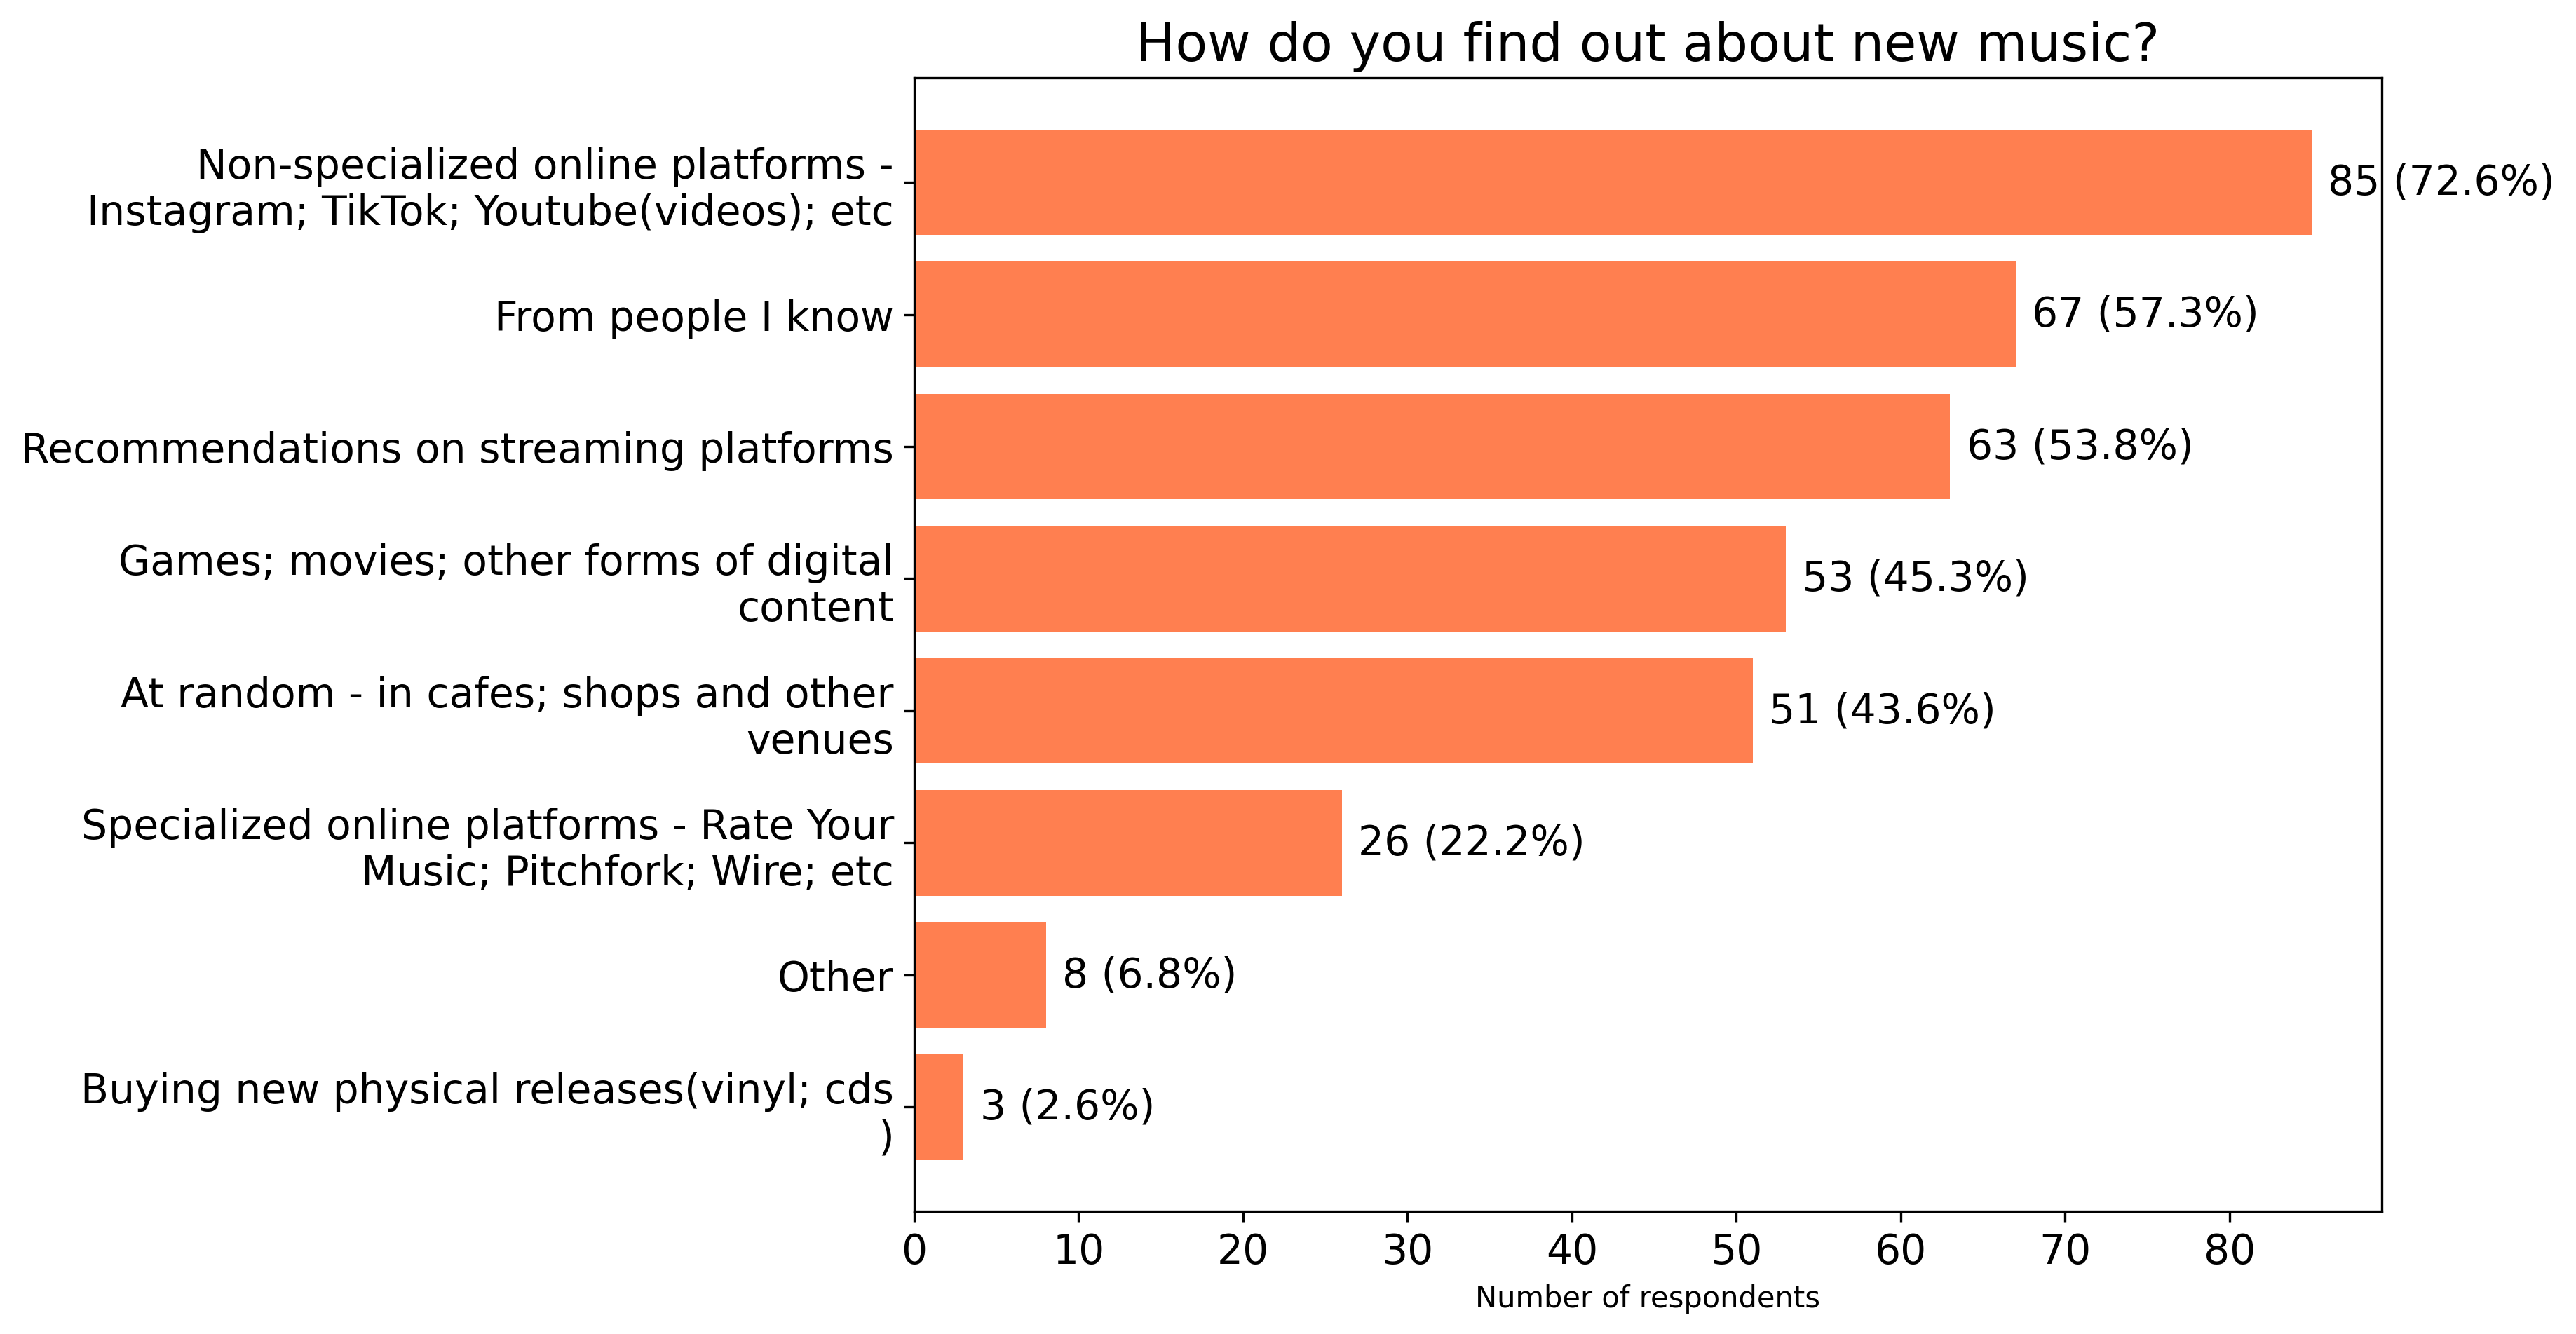
\includegraphics[height=0.4\textheight]{charts/discovery methods.png}
    \caption{Streaming platforms popularity}
    \label{fig:discovery_methods}
\end{figure}


\section{Streaming Services}
As can be seen in the ~\ref{fig:consumption_methods} and further confirmed by
the recent study of the International Federation of the Phonographic Industry\cite{music_stats_2024},
nowadays, the most prevalent way of music consumption
and discovery is through streaming services. Many options are available,
but only those that are both popular and have unique elements will be considered in this thesis.
The descriptions, rather than offering a general portrayal of each platform,
will focus on the service-specific features, including social elements.

\subsection{Spotify}
One of the most prominent social features on Spotify is the 'Spotify Jam'\cite{spotify_jam}.
It lets people create a collective song queue that is then synchronized among all connected users.
Moreover, volume, the order of songs, and other aspects of the playback can be controlled individually.
Another notable tool is the 'Blend' playlists\cite{spotify_recs}. These are playlists created automatically
between two people, which contain songs matching the audio preferences of both users.
Lastly, 'Friend Activity'\cite{spotify_friend_activ}, which shows what the people you follow are currently listening to,
and 'Listening Parties', which are live chats with a limited capacity,
that can be joined for a short time when new music is being released\cite{spotify_party_1,spotify_party_2}.

\subsection{VK Music}
VK Music is a music service integrated into the VK social network.
Consequently, it is possible to send songs and playlists via private messages and add audio materials to
posts in groups. VK Music also provides an 'Updates' tab, which is populated by the audio materials that
any followed user or group has added to their 'Liked' feed.

\subsection{SoundCloud}
SoundCloud is one of the few platforms that lets its users leave comments
and reactions on songs and playlists\cite{sc_comments,sc_reactions}.
In addition, each user has a feed consisting of personal uploads and
reposts of other's content\cite{sc_reposts}, which is visible when visiting their profile.

\subsection{Bandcamp}
Every Bandcamp user has a profile with four tabs: "collection", "wishlist", "followers", and "following".
The most interesting feature is under the `following` tab -- users can subscribe to available genres and then
specify the ones they want to showcase to others viewing their profile.
The "wishlist" tab is also noteworthy,
as Bandcamp’s model blends streaming with the traditional purchases of individual releases and
in this tab, the user can show what he is looking forward to listening to in the future.

The table~\ref{tab:social_features} summarizes the comparison between the features mentioned above.\\
\textbf{Difficulty} suggests the possible complexity of implementation.\\
\textbf{Mode} assumes the typical context in which the feature operates.\\
\textbf{Social Interaction Level} indicates user involvement when using the feature.\\


\begin{table}[ht]
    \caption{Comparison of Service‐Specific Social Features}
    \label{tab:social_features}
    \begin{tabular}{|l|l|c|c|c|}
        \hline
        \textbf{Feature}        & \textbf{Service} & \textbf{Difficulty} & \textbf{Mode}    & \textbf{Interaction Level} \\
        \hline\hline
        Spotify Jam             & Spotify          & High                & Group            & High                       \\
        \hline
        Blend playlists         & Spotify          & Medium              & Pair             & Low                        \\
        \hline
        Friend Activity         & Spotify          & Low                 & Pair             & Medium                     \\
        \hline
        Listening Parties       & Spotify          & Medium              & Group            & Medium                     \\
        \hline
        Music sending via chats & VK Music         & Medium              & Individual/Group & High                       \\
        \hline
        Embedding into posts    & VK Music         & Medium              & Individual/Group & Medium                     \\
        \hline
        Updates tab             & VK Music         & Low                 & Individual       & High                       \\
        \hline
        Comments                & SoundCloud       & Low                 & Group            & High                       \\
        \hline
        Reposts feed            & SoundCloud       & Low                 & Individual       & Medium                     \\
        \hline
        Genre following         & Bandcamp         & Medium              & Individual       & Low                        \\
        \hline
        Wishlist                & Bandcamp         & Low                 & Individual       & Low                        \\
        \hline
    \end{tabular}
\end{table}


\section{Forums, Blogs, and other Music Media}
Many different resources are gathered under these umbrella terms, from professional music review websites to
amateur and personal pages. Again, only widely used services that offer something remarkable are listed.

\subsection{Rate Your Music}

\begin{quote}
    'Rate Your Music is one of the largest music databases online. It is an incredible tool that
    can help you find and learn about new music to listen to.'\cite{ryt}.\\
\end{quote}
This website is one of the biggest platforms with user-created content.
Every member can write reviews and set ratings for music releases,
contribute to the extensive "wiki" consisting of genres, thematic lists and charts,
and connect to other members of the forum. However, the content is still moderated -- any post has
to be properly formatted and abide by the guidelines in order to appear on the website.

\subsection{2step.ru}
2step.ru is one of the better representatives of "old school" forums that is still active.
This is a country-specific resource, and as a consequence,
on top of providing the regular music and forum components, there are elements usually missing
from bigger portals. For example, a section about upcoming parties,
a page dedicated to local and upcoming DJs, and an ongoing list of recorded radio shows.\cite{2step}

\subsection{last.fm}
Last.fm is a music discovery and social networking service built around its "scrobbling" feature,
which automatically records every track played through connected players to the user’s profile,
creating an exhaustive listening history\cite{lastfm}.
Based on this data, Last.fm generates personalized recommendations and charts,
while tag-based navigation enables exploration of genres and user-curated collections.
Social interaction is fostered through friend lists, public groups for discussion, and the ability to comment
on artist and track pages. Additionally, an "Events" section aggregates concert listings and allows users to
indicate that they are interested or confirm that they are going and to add comments under each event post,
bridging online listening activity with real-world live music experiences.

In summary, these platforms illustrate the range of community-driven and data-driven approaches to music engagement
beyond pure streaming.
They highlight how social interaction and user-generated content can enrich interactions with music-related content.


\section{Other Platforms}

As mentioned earlier, one of the most interesting results of the survey is the high number of people
discovering music on platforms that are not focused on music.
Services like Instagram, YouTube, and TikTok—mainly used for sharing videos and other user content—have
become closely connected to how people find and listen to music.
In recent years, these platforms have started to promote music more directly by making it part of short,
easily shareable content that spreads quickly.
Instagram, for example, added a special audio tool that lets users include music in their 'Reels'\cite{inst_audio},
helping songs reach more people through visual content.
YouTube automatically finds songs used in videos and shows them in the description, making finding and listening to them easier.
TikTok has had an even bigger impact -- many songs have gone viral and later became hits in charts and streaming apps
because people use them in popular videos. These are often called “TikTok hits.”

This shows that big platforms are not just reacting to users’ interest in music -- they
actively help promote it by connecting songs with content that people want to watch and share.

And for example, an integration with such services can be a big plus for the platform, improving the user experience
when it comes to exploring the songs they like.

\section*{Summary}
As can be seen, there are numerous instruments available across the Internet.
However, services that focus on the actual audio delivery often lack features stretching beyond that,
forcing users to use multiple platforms in order to meet their needs. This project aims to bridge that gap,
particularly by enhancing users' potential for social interaction.

Based on the research done in the previous and current chapters, these social features were chosen for implementation,
as they are both easy to implement and provide a high level of social interaction:

\begin{itemize}
    \item Comments under audio content.
    \item Individual posts and a feed with posts of others.
    \item Friend listening activity.
    \item Latest content added by friends.
\end{itemize}

These and further requirements for the application are listed in the following chapter - \nameref{chap:specification}.